\documentclass[11pt]{article}
\usepackage{acl}

\usepackage{times}
\usepackage{latexsym}
\usepackage{amsmath}
\usepackage{amssymb}
\usepackage{graphicx}
\usepackage{booktabs}
\usepackage{url}
\usepackage{microtype}

\title{Reader-faithfulness: What a Book Assistant May Know at Chapter $c$, and the Two Ways It Breaks That Promise}

\author{Anonymous ACL Submission}

\begin{document}
\maketitle

\begin{abstract}
A book assistant that answers ``as of chapter $c$'' makes a promise to the reader: nothing it says may depend on chapters after $c$. We call this \textbf{reader-faithfulness} and define it as invariance of the output at position $c$ to the rest of the volume. The promise can be broken through two channels that look different but violate the same contract. In \textbf{Channel 1, parametric memory}, the language model inside the system has already read the book, so a prompt truncated at chapter $c$ still elicits the later reveal; we measure this as name-keyed premature identity naming, original names against consistently replaced names, with an unseen-text control and a cue-preserving pseudonym control. In \textbf{Channel 2, derivation look-ahead}, the pipeline around the model stores a derived fact stamped with the chapter where the character first appears but computed from up to twelve later chapters, so a query filtered to chapter $c$ returns values that a build over chapters up to $c$ does not hold. Truncating the input and rebuilding gives an exact oracle for this channel. On a deployed narrative knowledge graph the served gender differs from the prefix build for 6.0\% of 685 character-cuts of three translated web novels, 4.5\% of 179 on two English originals, and 9.2\% to 17.1\% of pairs on a synthetic volume with known truth. Versioning each derived fact by its evidence horizon removes divergence entirely (0 in all real, public-domain, and synthetic runs). The two channels need different instruments, because truncation cannot see a memory held in the weights, and they compose, because a derivation that calls a model inherits the model's memory.
\end{abstract}

\section{Introduction}

Position-aware reading assistants are now a product category. Kindle's ``Ask this Book'' answers ``up to your current reading position'', and recent industry disclosures describe tagging facts with progress points and retrieving only those prior to reader progress. The premise is simple and valuable: a reader in the middle of a mystery should be able to ask who a character is without learning reveals from chapter 40.

However, existing systems do not verify that the filter's inputs are free of later information. There are at least two ways they violate this contract:
\begin{itemize}
    \item \textbf{The model knows the book (Channel 1).} If the assistant uses a language model to link an alias to an identity, truncating the context at chapter $c$ does not prevent a model that memorized the novel from naming an unrevealed identity.
    \item \textbf{The pipeline's derived facts look ahead (Channel 2).} If the assistant derives facts (e.g., gender, archetype, persona traits) from evidence accumulated over multiple chapters, stamping them at the first mention serves future information to early readers.
\end{itemize}

This paper formalizes reader-faithfulness, measures both channels on a deployed narrative graph, reports the repairs and their trade-offs, and highlights remaining challenges.

\section{Setting: A Volume, a Reader Position and a Pipeline}

A volume consists of chapters $1 \dots n$. A reader at position $c$ has read chapters $1 \dots c$. The audited system is EchoTales, a pipeline building a bitemporal narrative knowledge graph with discourse order, story time, and \textbf{knowledge time} (the position at which a reader could know a fact), queried via $\texttt{state\_of}(\text{READER}, c)$.

Processing is \textbf{volume-first}: the entire volume is ingested at once, meaning write timestamps carry no knowledge-time information. Knowledge time must be reconstructed from evidence position. The store contains both single-passage facts and multi-chapter derived traits.

\section{Definition and Formal Note}

\subsection{Reader-faithfulness}

Let $S$ be a system that, given volume $x = (x_1, \dots, x_n)$ and position $c$, outputs $S(x, c)$.
\begin{quote}
\textbf{Definition (Reader-faithfulness).} $S$ is reader-faithful if for every position $c$ and every pair of volumes $x, x'$ with identical prefixes $x_{\le c} = x'_{\le c}$, $S(x, c) = S(x', c)$.
\end{quote}
For deterministic systems, this implies an exact operational test: \textbf{truncate and rebuild}.

When $S(x, c; \theta)$ contains learned parameters $\theta$:
\begin{itemize}
    \item \textbf{Input channel (Channel 2):} $S(x, c; \theta)$ is invariant to $x_{>c}$ for fixed $\theta$.
    \item \textbf{Parameter channel (Channel 1):} $S(x_{\le c}, c; \theta)$ does not depend on what $\theta$ encodes about $x_{>c}$.
\end{itemize}

\subsection{The Part of Channel 2 That is Elementary}

A deterministic derivation $D$ maps chapter evidence to values. The reference at cut $k$ is $r_k = D(x_1 \dots x_k)$. A policy serves $s_k$; divergence is $\sum \mathbb{I}(s_k \ne r_k)$. The evidence horizon is $H = \max R(x_1 \dots x_n)$.
\begin{itemize}
    \item \textbf{P1 (Screen):} All divergence lies in the exposure window $k < H$.
    \item \textbf{P3 (Hiding vs. doing nothing):} Naive hiding beats status quo only if fewer in-window prefixes hold the final value than the neutral one.
    \item \textbf{P4/P5 (Versioning):} Serving $s_k = r_k$ achieves divergence 0.
    \item \textbf{P6 (Policy guarantee):} The guarantee belongs to the policy wrapper, not to $D$.
\end{itemize}

\section{Related Work}

\paragraph{Position-aware assistants and temporal graphs.} Zep/Graphiti \citep{zep2025graphiti} maintains bi-temporal graphs where the second timeline is ingestion order; under whole-volume ingestion, knowledge time must be explicitly derived.
\paragraph{Memorisation and renaming controls.} TimeChara \citep{timechara2024} showed parametric plot leakage in role-play. SynthWorlds \citep{synthworlds2026} and \citet{jiang2024memorization} use entity replacement to decouple memorization from reasoning.
\paragraph{Stream processing and point-in-time rules.} The Dataflow model \citep{dataflow2015} separates event time from processing time; our horizon versioning adapts accumulating panes to reader knowledge time.

\section{Channel 2: Derivation Look-Ahead}

\subsection{Method}
We evaluate the persona stage of EchoTales. We compare $\texttt{state\_of}(\text{READER}, k+0.5)$ from a whole-volume build against a prefix-only build over chapters $\le k$. Across three translated web novels (Lord of the Mysteries, Omniscient Reader's Viewpoint, Reverend Insanity), we evaluate 685 character-cuts, alongside two English public-domain novels (179 character-cuts) and a synthetic volume.

\subsection{Results}
\begin{itemize}
    \item \textbf{R1. Real defect:} Status-quo divergence occurs in 6.0\% of 685 web novel character-cuts (41/685) and 4.5\% of English originals (8/179).
    \item \textbf{R2. Screen soundness:} 0 divergences occur outside the static exposure screen window.
    \item \textbf{R3. Spoilers vs. supported facts:} Only 1.7\%--3.5\% of character-cuts are premature disclosures; the remainder were already supported by the text prefix.
    \item \textbf{R4. Horizon repair:} Horizon-versioned stamping drives divergence to exactly 0 of 685 cuts across all datasets.
    \item \textbf{R5. Hiding fails:} Naive hiding diverges on 82 of 289 cuts (worse than doing nothing: 23/289).
    \item \textbf{R6. Anchored cue:} Recovers 97\% of withheld correct values at a 1.2\% error rate on web novels.
\end{itemize}

\subsection{The Model Path of the Same Stage}
When characters have $\ge 25$ mentions, an LLM path is called. The prompt given identical prefix text yields 0 noise floor, but the gate condition ($N \ge 25$ over the full volume) causes prominence leakage in 50/296 pairs. Deciding the gate on prefix counts eliminates this look-ahead ($50 \to 0$).

\section{Channel 1: Parametric Memory (Skeleton)}

\subsection{Method}
We formulate an alias-reveal task: a passage introduces a disguised character (``the masked guest''), candidates include the true identity and decoys, and the question is asked prior to the reveal. Under Arm A (original names), memorized models prematurely name the identity. Under Arm B (letter cipher) and Arm B3 (cue-preserving pseudonyms matched by gender and name type), parametric memory is disrupted. Controls include an unseen-text control (E2) and title-assisted probes.

\begin{figure}[t]
\centering
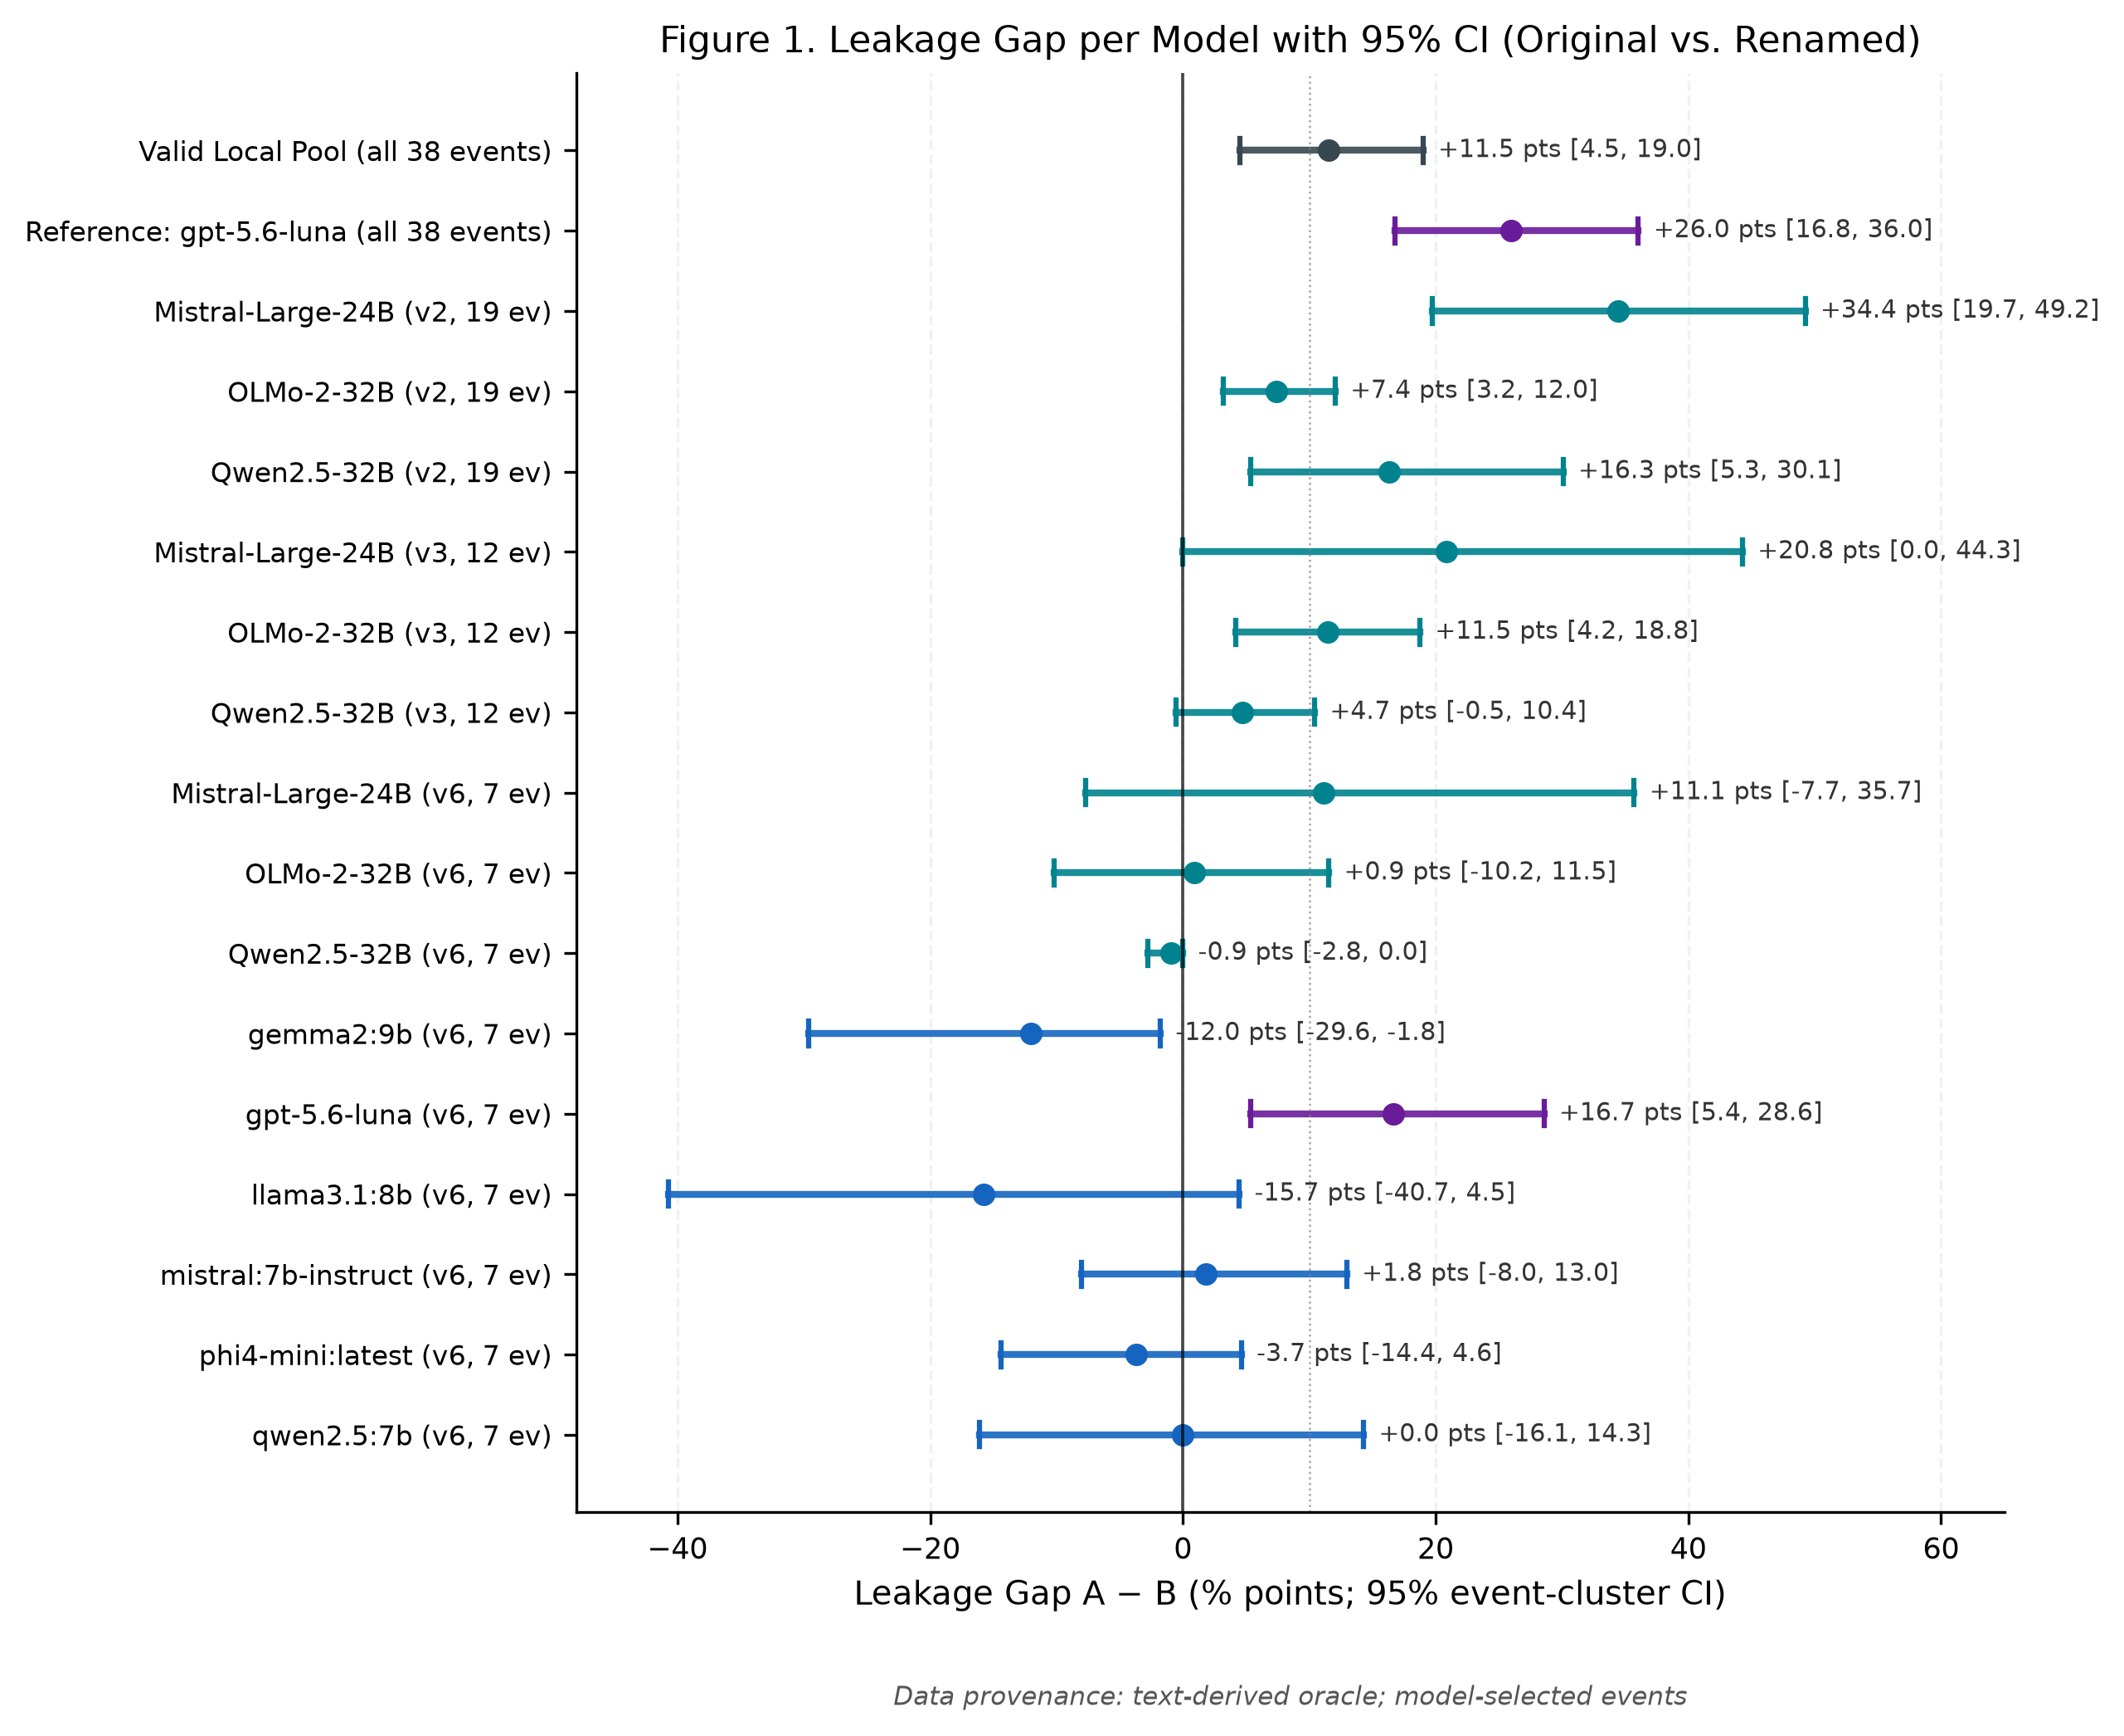
\includegraphics[width=\linewidth]{../figures/rf/fig_leakage_gap_per_model.png}
\caption{\textbf{Figure 1: Name-keyed leakage gap per model with 95\% CI.} Original names minus renamed cipher ($A - B$) across API reference, remote 24B--32B models, and local models. Provenance: text-derived oracle; model-selected events.}
\label{fig:leakage_gap}
\end{figure}

\begin{figure}[t]
\centering
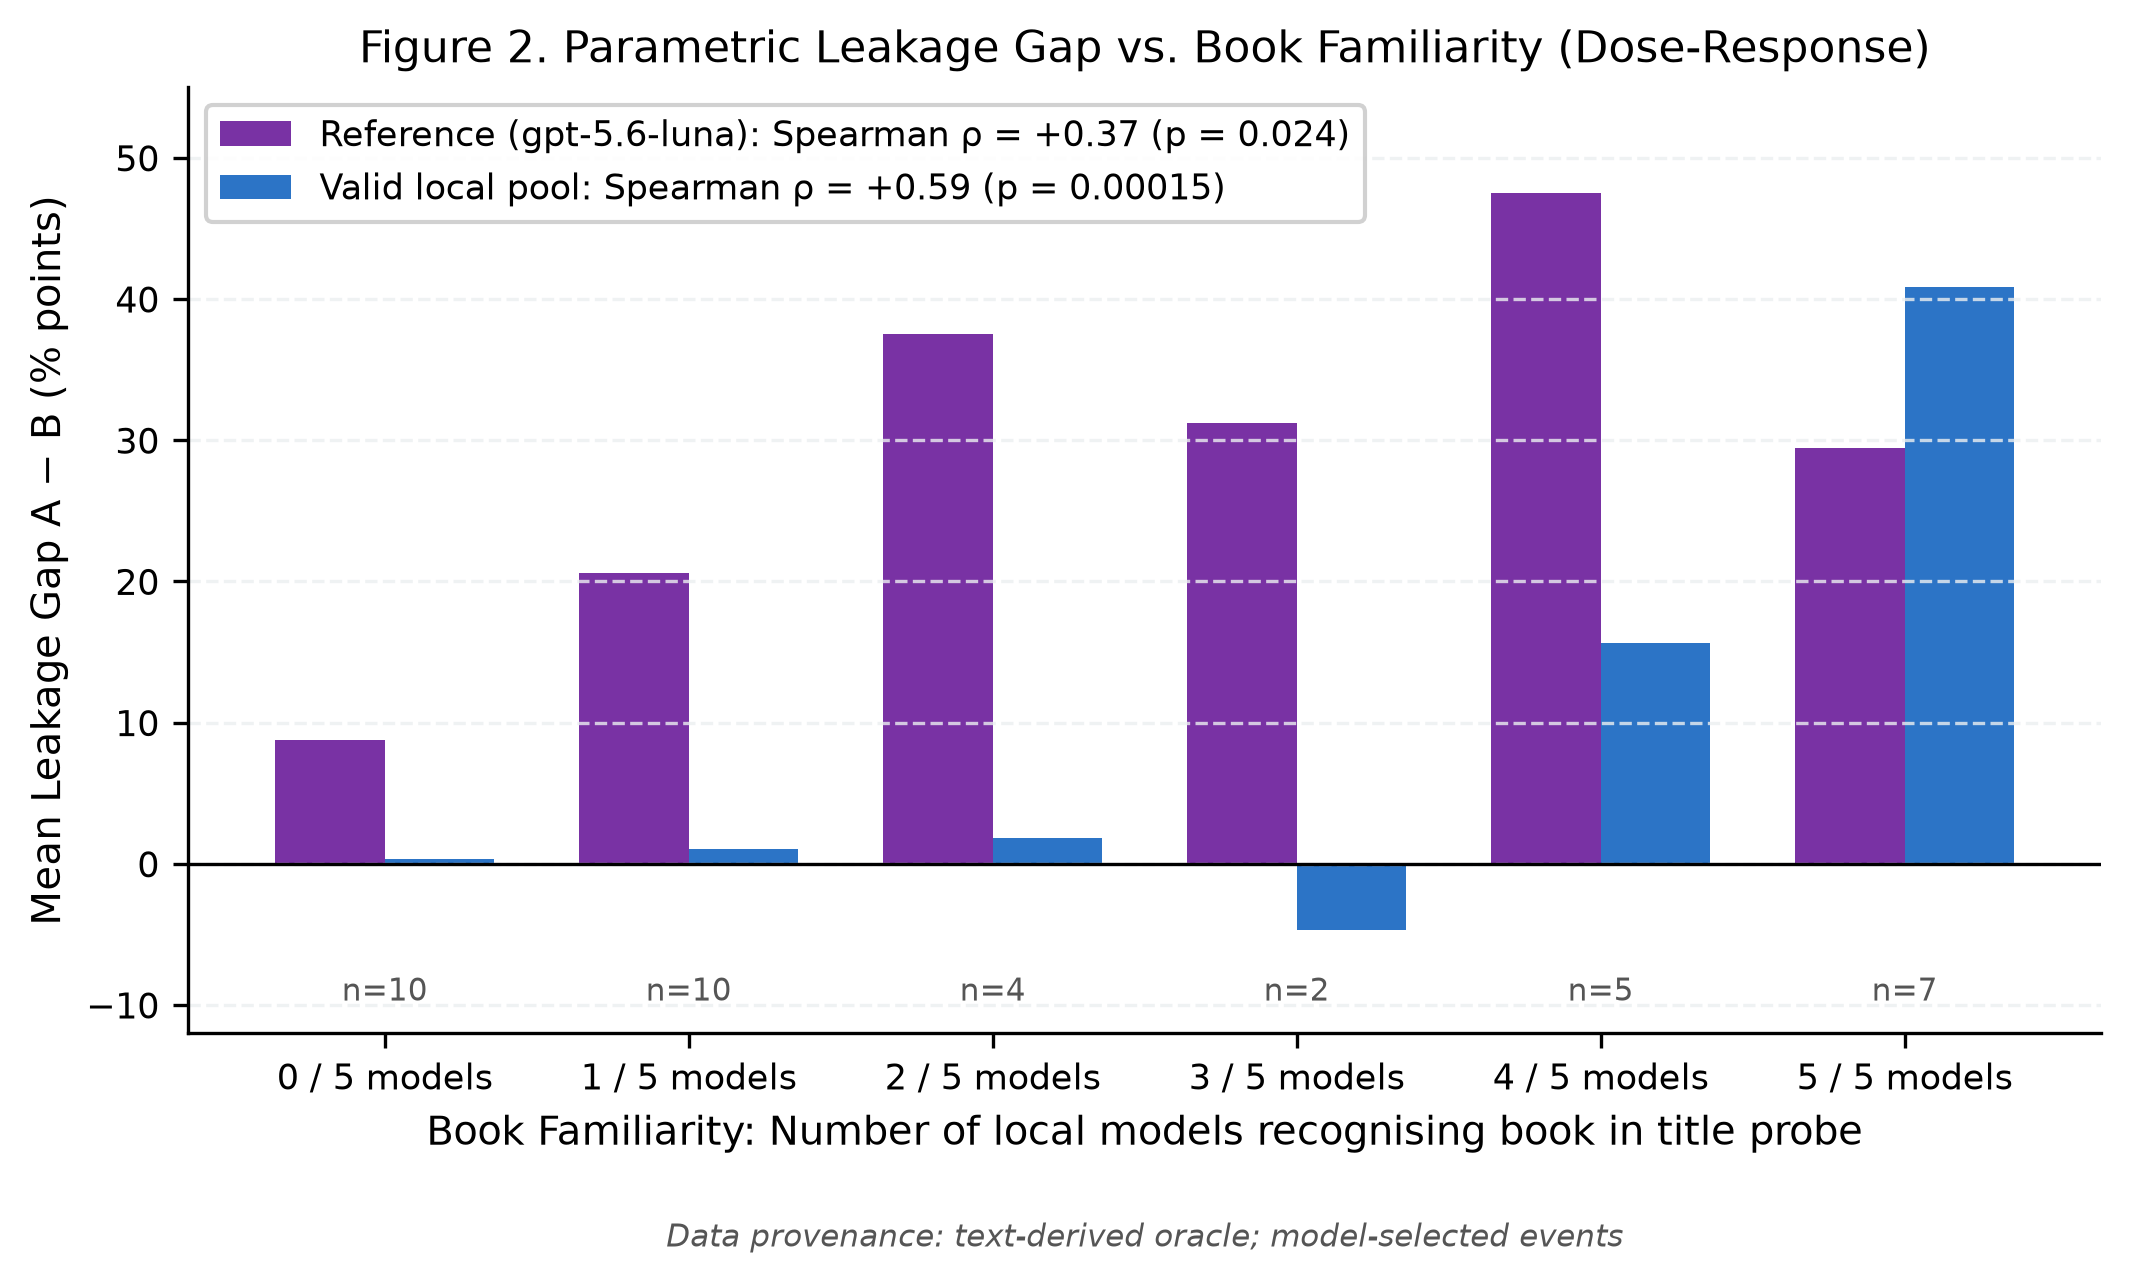
\includegraphics[width=\linewidth]{../figures/rf/fig_dose_response.png}
\caption{\textbf{Figure 2: Parametric leakage gap vs. book familiarity.} Mean leakage gap rises monotonically with the number of local models recognising the novel in title probes. Provenance: text-derived oracle; model-selected events.}
\label{fig:dose_response}
\end{figure}

\subsection{Results}
Figures \ref{fig:leakage_gap} through \ref{fig:unseen_text_control} present the experimental findings:

\paragraph{Leakage gap per model.} As shown in Figure \ref{fig:leakage_gap}, reference model \texttt{gpt-5.6-luna} exhibits a +26.0 pt gap ($p < 10^{-4}$) across 38 events. Remote models (Mistral-Large-24B, Qwen2.5-32B, OLMo-2-32B) show significant positive leakage on v2 and v3 sets, while small local models on fresh v6 books show lower or unreplicable gaps.

\paragraph{Dose-response.} Figure \ref{fig:dose_response} illustrates that leakage tracks book fame. For books recognized by 0 local models, local pool leakage is +0.3 pts ($n=10$); for books recognized by all 5 models, leakage reaches +40.8 pts ($n=7$, Spearman $\rho = 0.586$, $p = 0.00015$).

\begin{figure}[t]
\centering
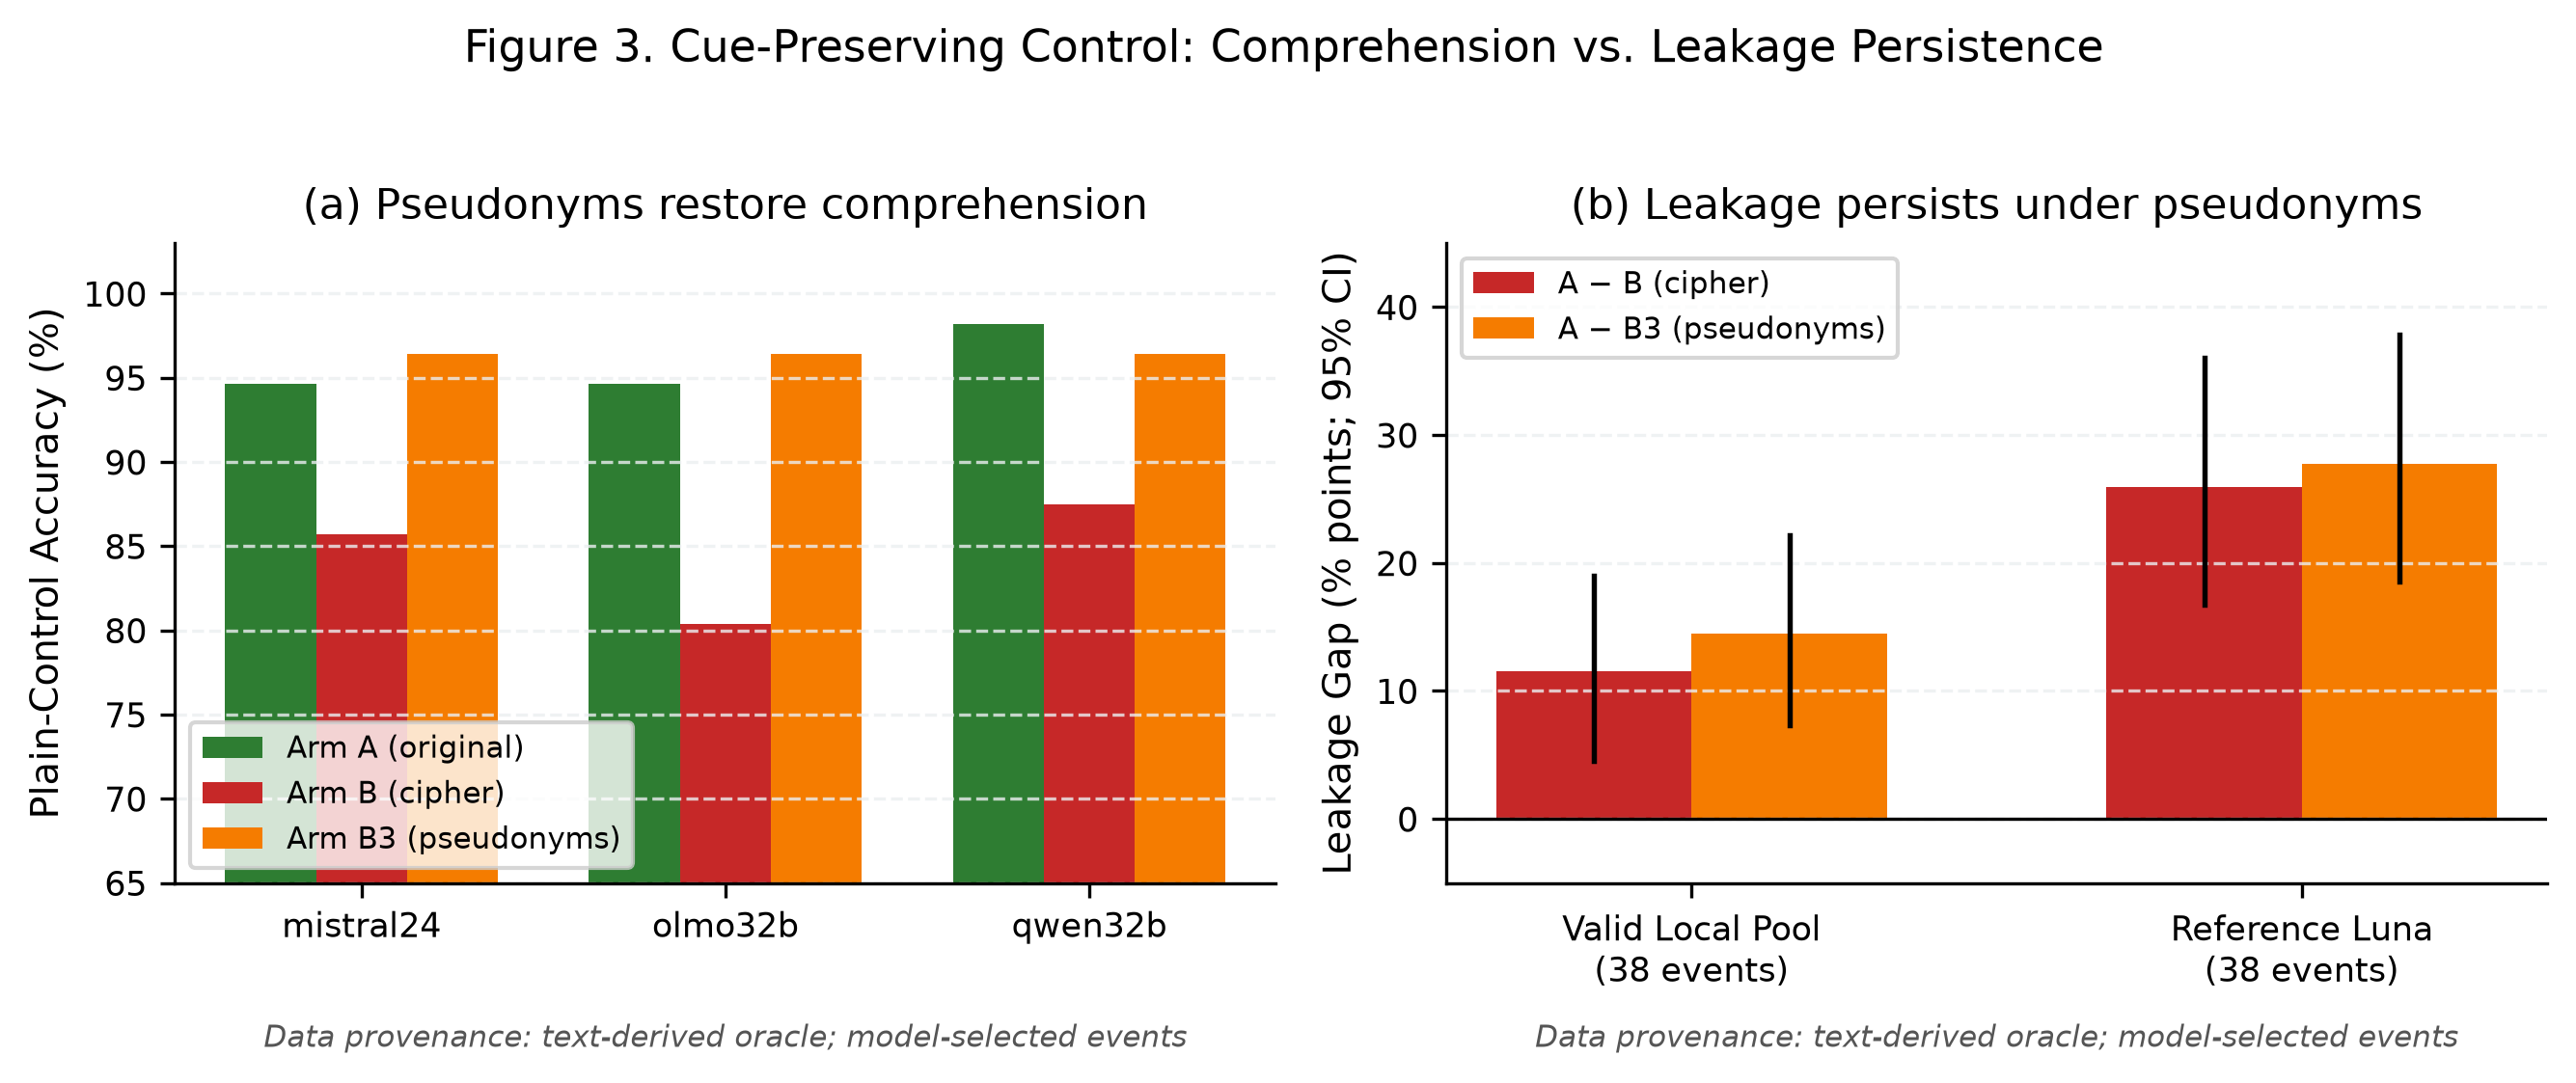
\includegraphics[width=\linewidth]{../figures/rf/fig_cue_preserving_bars.png}
\caption{\textbf{Figure 3: Cue-preserving control (Arms A, B, B3).} (a) Pseudonyms restore comprehension accuracy to original levels. (b) Premature naming gap persists under pseudonyms, confirming parametric memory rather than lost name cues. Provenance: text-derived oracle; model-selected events.}
\label{fig:cue_preserving}
\end{figure}

\begin{figure}[t]
\centering
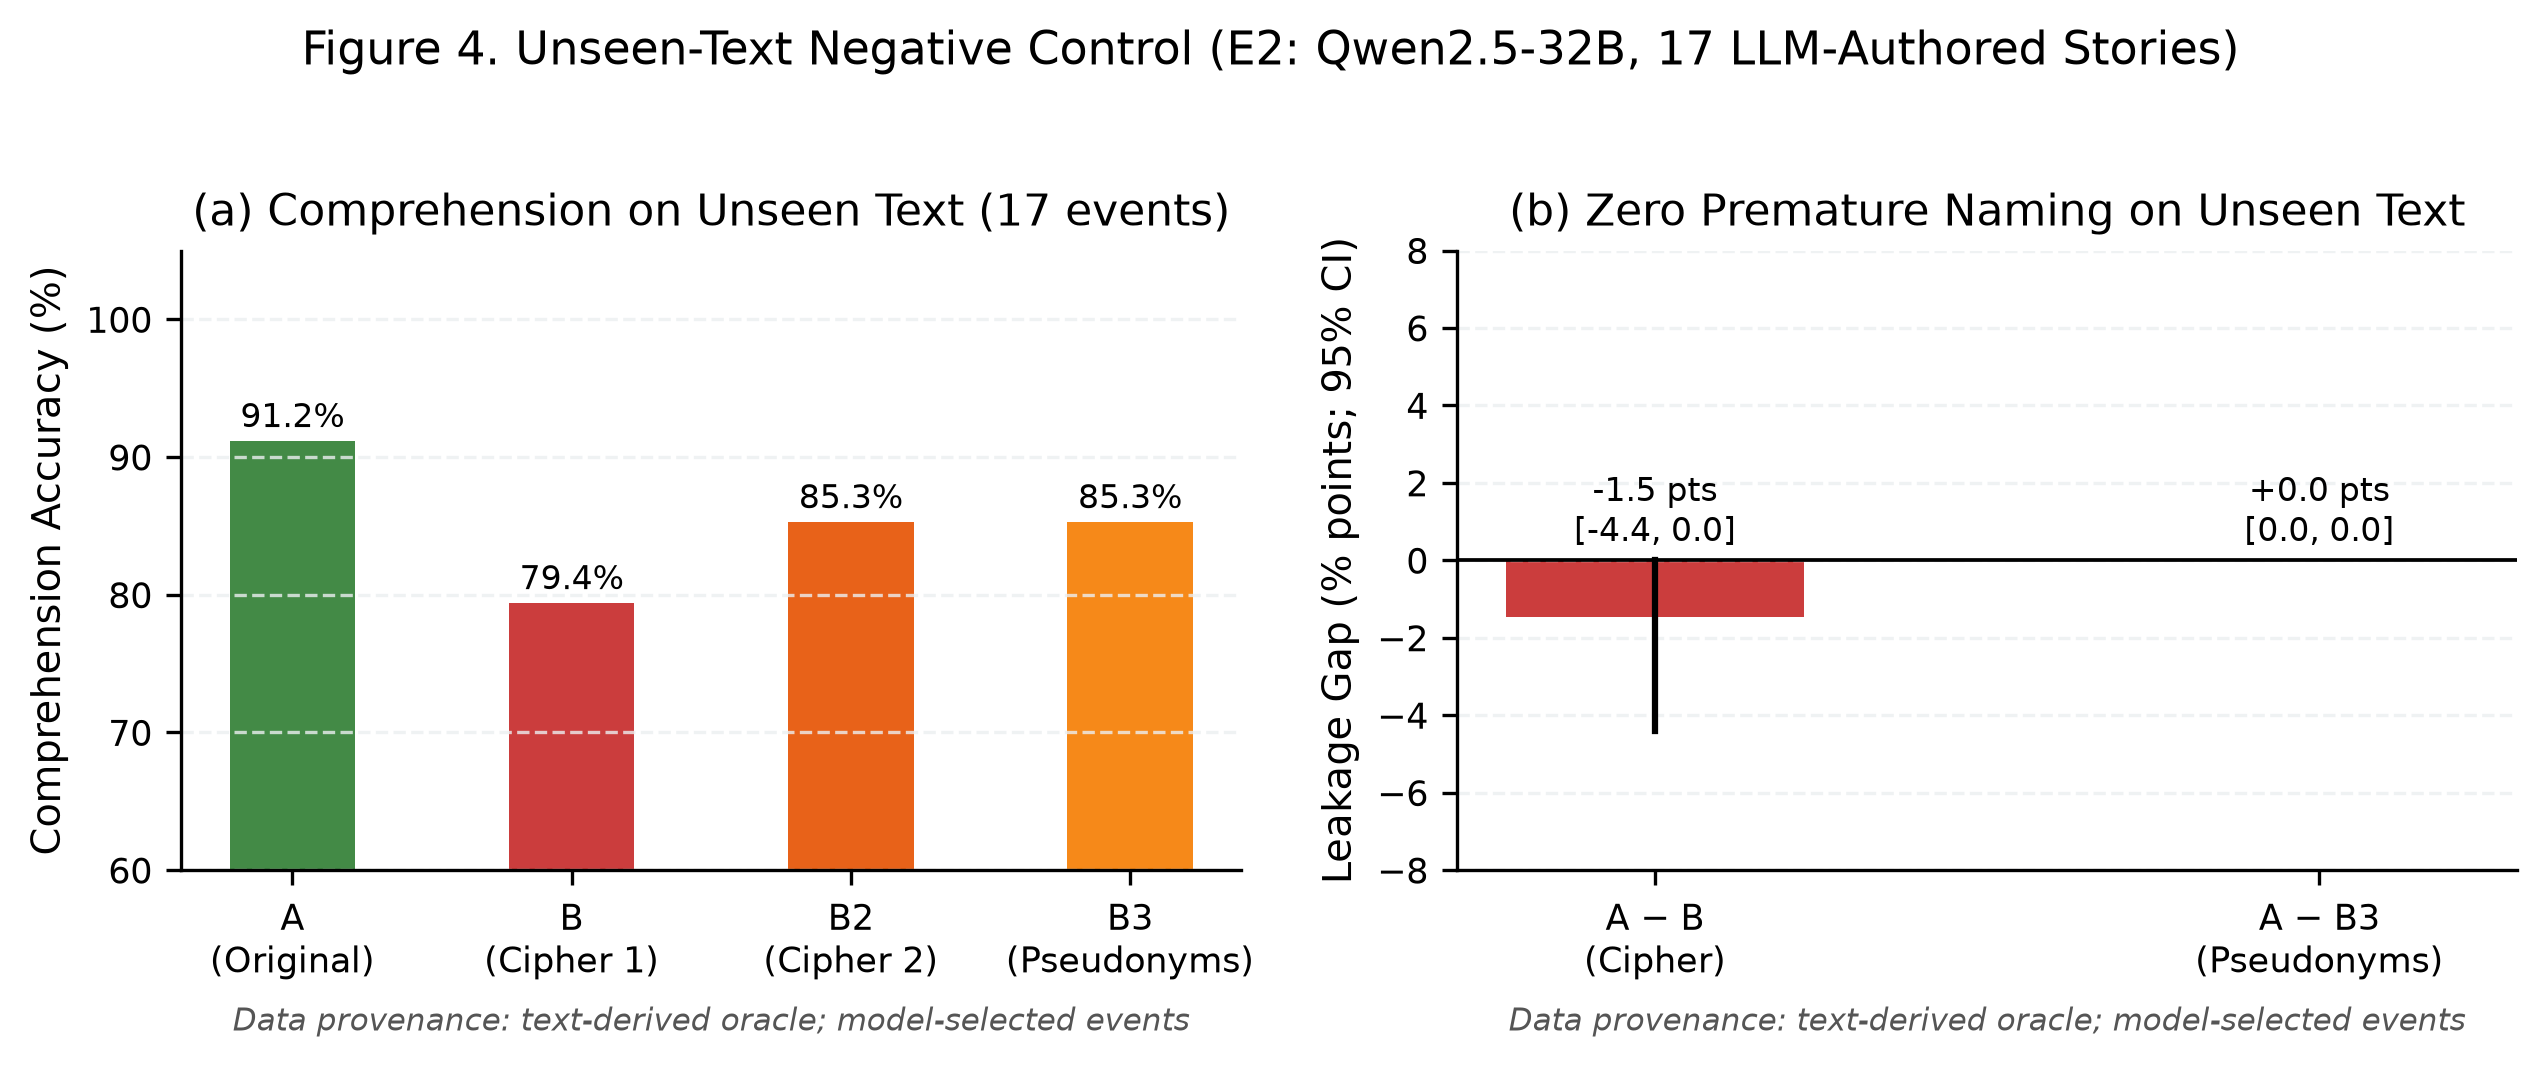
\includegraphics[width=\linewidth]{../figures/rf/fig_unseen_text_control.png}
\caption{\textbf{Figure 4: Unseen-text negative control (E2).} On 17 newly authored stories absent from pretraining weights, the leakage gap is 0.0 pts (95\% CI [0.0, 0.0]). Provenance: text-derived oracle; model-selected events.}
\label{fig:unseen_text_control}
\end{figure}

\paragraph{Cue-preserving pseudonyms.} Figure \ref{fig:cue_preserving} demonstrates that natural pseudonyms (Arm B3) restore plain-control comprehension (e.g., 96.4\% accuracy) while leaving the premature naming gap fully intact (+14.5 pts pooled), refuting the hypothesis that Arm B's gap is caused by syntactic disruption.

\paragraph{Unseen-text control.} Figure \ref{fig:unseen_text_control} confirms that on 17 LLM-authored stories never seen during pretraining, the leakage gap is zero (-1.5 pts under cipher, 0.0 pts under pseudonyms).

\subsection{What Channel 1 Cannot Be}
Renaming bounds name-keyed parametric memory; plot-keyed or phrase-keyed memories are unmeasured. The numbers reflect the specific models tested.

\section{Repairs and Trade-offs}

\begin{table*}[t]
\centering
\small
\begin{tabular}{lp{6.5cm}p{6.5cm}}
\toprule
\textbf{Dimension} & \textbf{Channel 2: Derivation Look-Ahead} & \textbf{Channel 1: Parametric Memory} \\
\midrule
\textbf{Cause} & Derived fact stamped earlier than evidence horizon & Model weights encode volume suffix \\
\textbf{Instrument} & Truncate-and-rebuild exact oracle & Renaming controls, unseen-text probe \\
\textbf{Input repairable?} & Yes: recompute from prefix & No: suffix knowledge resides in parameters \\
\textbf{Repair tested} & Horizon versioning; anchored cue; prefix gate & Pseudonymization, evidence-gated linking \\
\textbf{Guarantee} & Divergence 0 for prefix-causal derivations & Name-keyed memory bounded \\
\textbf{Price} & Withholds supported values until horizon & Extraction complexity, potential cue loss \\
\bottomrule
\end{tabular}
\caption{Comparison of failure channels, instruments, guarantees, and trade-offs.}
\label{tab:repairs}
\end{table*}

Table \ref{tab:repairs} summarizes the contrast between the two channels. The two channels compose: a pipeline can be completely faithful in Channel 2 yet break reader-faithfulness via Channel 1.

\section{Combined View of the Evidence}

The combined evidence demonstrates that position-filtered narrative assistants face simultaneous vulnerabilities in data derivation and model weights. Both must be audited and repaired to ensure reader-faithfulness.

\section{Limitations}

\begin{itemize}
    \item \textbf{Label provenance:} Channel 1 uses text-derived oracles without owner-verified labels. Channel 2 labels rely on model annotators and system-internal rebuilds.
    \item \textbf{Scope:} Evaluated on five full volumes (three translated web serials, two English public-domain novels), plus synthetic benchmarks.
    \item \textbf{Unrepaired elements:} Body splits and whole-volume prominence features remain subject to architectural trade-offs.
\end{itemize}

\section{Conclusion}

Reader-faithfulness guarantees that an assistant's answers at chapter $c$ depend strictly on chapters $\le c$. We identified two distinct mechanisms breaking this promise: derivation look-ahead (Channel 2) and parametric memory (Channel 1). Horizon versioning solves Channel 2 with provable zero divergence. Controlled renaming exposes and measures Channel 1. Robust position-aware reading systems require defending against both channels.

\appendix

\section{Where Each Number Comes From}
Channel 2 figures derive from the system-internal audit in \texttt{docs/research/PREFIX\_FAITHFULNESS/REPORT.md}. Channel 1 numbers derive from pooled evaluations in \texttt{data/eval/chimera/pd\_final\_pooled.json}, \texttt{pd\_dose\_response.json}, remote GPU analysis files, and confirmatory experiment \texttt{confirm/e2/analysis.json}.

\section{Placeholders for the Main Session}
Numbers for Channel 1 reflect the finalized evaluation artifacts committed on this branch.

\bibliographystyle{acl_natbib}
\bibliography{custom}

\end{document}
